\documentclass[10pt]{beamer}
\usepackage[slovak]{babel}
\usetheme[progressbar=frametitle]{metropolis}
\usepackage{appendixnumberbeamer}
\usepackage{booktabs}
\usepackage[scale=2]{ccicons}
\usepackage{pgfplots}
\usepgfplotslibrary{dateplot}
\usepackage{xspace}
\newcommand{\themename}{\textbf{\textsc{metropolis}}\xspace}



\title{Porovnanie typov rekurentných neurónových sietí z hľadiska hĺbky pamäte}
\subtitle{Diplomová práca}
% \date{\today}
\date{}
\author{Jaroslav Ištok}
%\institute{Faculty of Mathematics Physics and Informatics Comenius University Bratislava}
% \titlegraphic{\hfill\includegraphics[height=1.5cm]{logo.pdf}}

\begin{document}

\maketitle

\begin{frame}{Obsah}
  \setbeamertemplate{section in toc}[sections numbered]
  \tableofcontents[hideallsubsections]
\end{frame}


\section{Elmanova rekurentná neurónová sieť}

\begin{frame}[fragile]{Elmanova rekurentná neurónová sieť}
\begin{itemize}
\item Architektúra siete 
\item Trénovanie pomocou algoritmu spätného šírenia chyby cez čas
\item Kontextová vrstva neurónov (kontextové neuróny)
\item Možnosti využitia 
\end{itemize}
\end{frame}

\begin{frame}[fragile]{Elmanova rekurentná neurónová sieť}

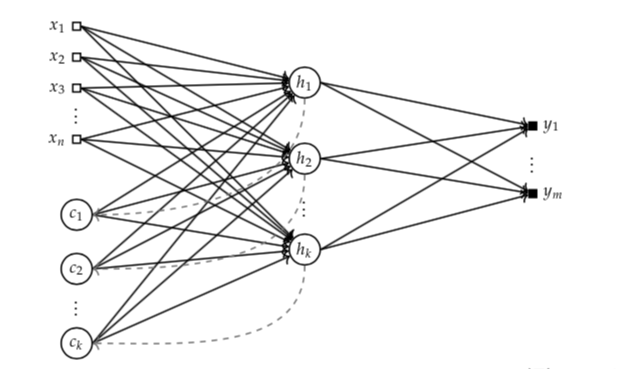
\includegraphics[width=\textwidth]{elman}

\end{frame}

\section{Samoorganizujúca sa mapa}
\begin{frame}[fragile]{SOM}

\begin{itemize}
  \item pojem samoorganizujúca sa mapa
  \item biologicky motivovaný model
  \item učenie so súťažením
  \item učenie bez učiteľa
  \item zhlukovanie dát
  \item zachovanie topologických vlastností dát
\end{itemize}

Hľadanie víťaza
\begin{equation*}
i^* = argmin_i||x-w_i|| 
\end{equation*}

Aktualizácia váh
\begin{equation*}
w_i(t+1) = w_i(t) + \alpha(t)h(i^*, i)([x(t) - w_i(t)]
\end{equation*}

\end{frame}

\section{Rekurentná SOM}

\begin{frame}[fragile]{Rekurentná SOM}
Je to samoorganizujúca sa mapa, 
\begin{itemize}
\item RecSom - kontextom je kópia aktivácii neurónov z predchádzajúceho kroku
\item Veľké množstvo atribútov
\end{itemize}
Aktualizácia váh neurónov
\begin{equation*}
w_i(t+1) = w_i(t) + zh_{ik}[s(t) - w_i(t)]
\end{equation*}
\begin{equation*}
c_i(t+1) = c_i(t) + zh_{ik}[y(t - 1) - c_i(t)]
\end{equation*}
\begin{equation*}
y_i=exp(-d_i)
\end{equation*}
Vzdialenosť
\begin{equation*}
d_i(t) = \alpha||x(t)-w_i||^2 + \beta||r(t)-c_i||^2
\end{equation*}
Rekurzívny kontext
\begin{equation*}
r(t)=[y_i(t-1),...,y_N(t-1)]
\end{equation*}
\end{frame}

\section{Merge SOM}

\begin{frame}[fragile]{Merge SOM}

\begin{itemize}
\item V merge SOM kontext nie je kópia celej mapy z predchádzajúceho kroku
\item Kontextom sú vlastnosti víťazného neurónu z predchádzajúceho kroku
\item Menej parametrov ako pri rekurzívnej SOM
\end{itemize}
Aktualizácia váh
\begin{equation*}
\Delta w_i = \gamma_{1} \cdot h_{\sigma}(d_{N}(i, I_{t})) \cdot (x^t - w^i)
\end{equation*}
\begin{equation*}
\Delta c_i = \gamma_{2} \cdot h_{\sigma}(d_{N}(i, I_{t})) \cdot (c^t - c^i)
\end{equation*}

Vzdialenosť
\begin{equation*}
d_i(t) = (1-\alpha) \cdot ||x^t - w^i||^2 + \alpha \cdot ||c^t - c^i||^2
\end{equation*}

Rekurzívny kontext
\begin{equation*}
c^t = (1 - \beta) \cdot w^{I_{t-1}} + \beta \cdot c^{I_{t-1}}
\end{equation*}
\end{frame}

\section{Určovanie pamäťovej hĺbky}
\begin{frame}[fragile]{Určovanie pamäťovej hĺbky}a

\begin{itemize}
\item Vstup - sekvencia písmen (znakov)
\item Každý neurón má navyše množinu, v ktorej si pamätá pre ktoré vstupy bol víťazom
\item Nezapamätá si iba aktuálny vstup ale aj $k$ posledných vstupov, tzv. posuvné okno
\item Na konci každej epochy trénovania zistíme dĺžku najdlhšej spoločnej podpostupnosti pre každý neurón
\item Tým získame pamäťovú hĺbku pre jednotlivé neuróny
\item Keď spravíme vážený priemer pamäťových hĺbok pre všetky neuróny v sieti dostaneme pamäťovú hĺbku pre celú sieť
\item Toto číslo budeme používať ako mieru pamäťovej hĺbky pre SOM 
\end{itemize}

\end{frame}

\begin{frame}[fragile]{Ukážka receptívneho poľa}
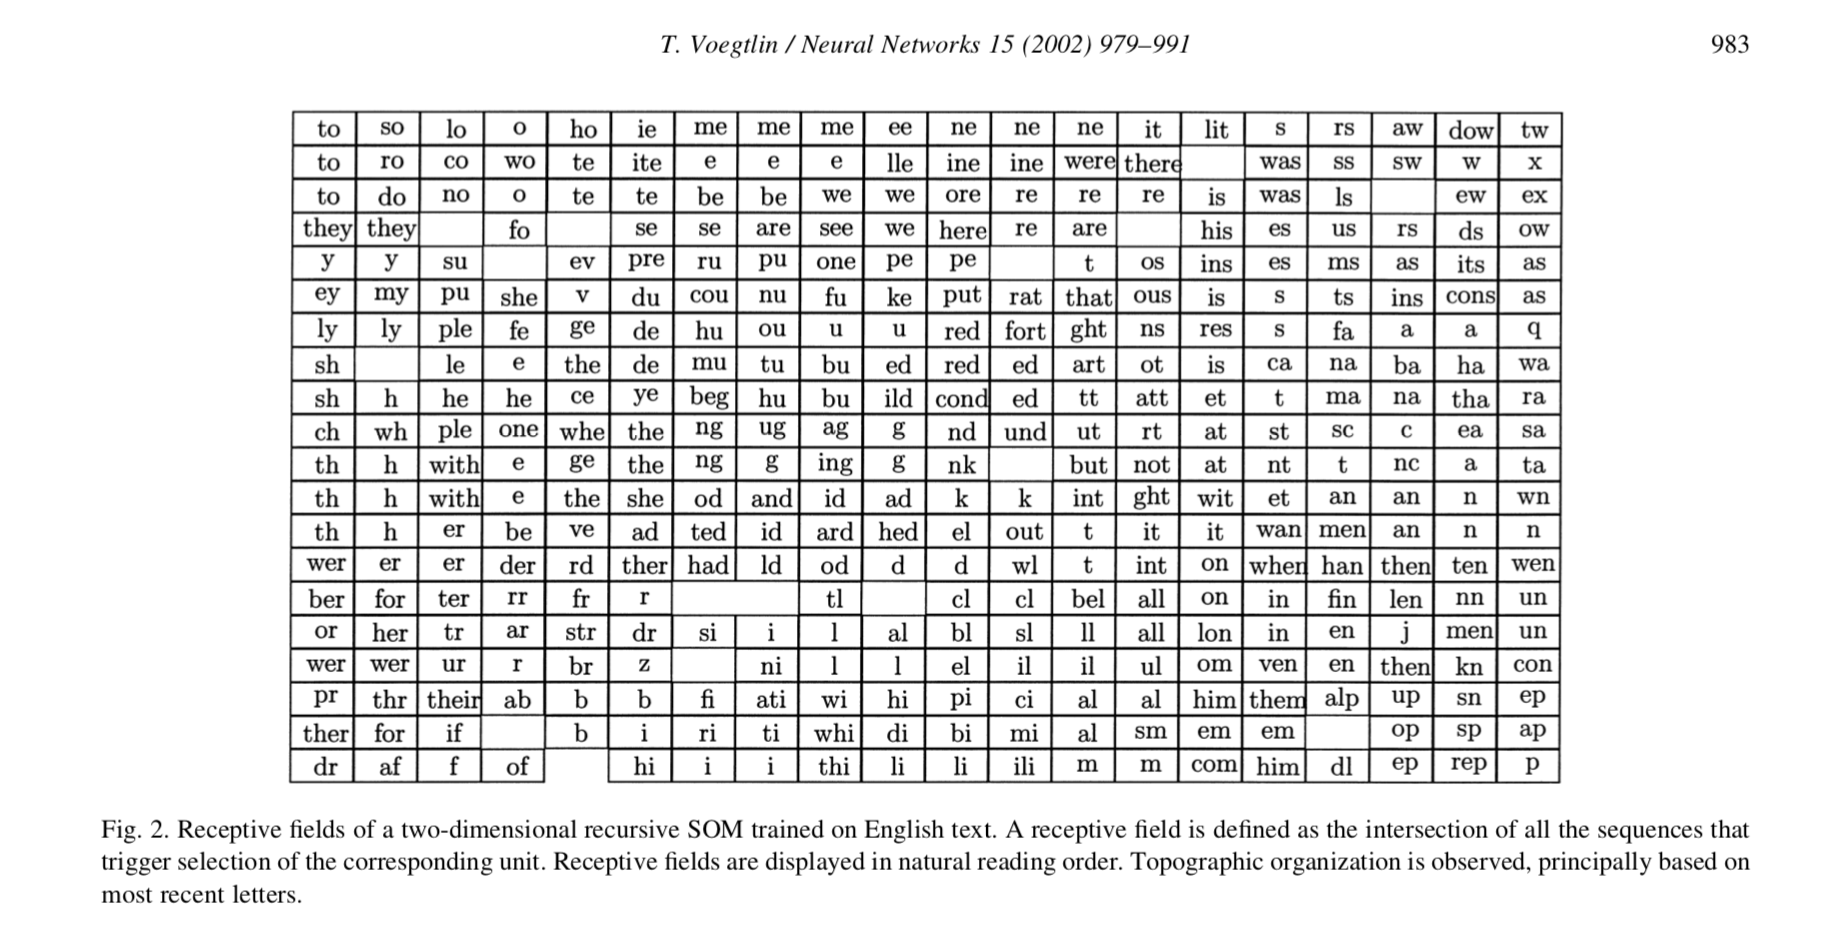
\includegraphics[width=\textwidth]{receptive_field}
\end{frame}

\section{Implementácia}
\begin{frame}{Implementácia}

\begin{itemize}
  \item Vlastná implementácia jednotlivých druhov neurónových sietí
  \item Python + Numpy
  \item Algoritmus hľadania najdlhšej spoločnej podpostupnosti viacerých podpostupností
  \item Implementácia posuvného okna
\end{itemize}
\end{frame}


\section{Čo ďalej?}
\begin{frame}{Čo ďalej?}
  \begin{itemize}
    \item Implementácia algoritmu spätného šírenia chyby v čase
    \item Vymyslieť spôsob ako merať pamäťovú hĺbku v Elmanovej sieti
    \item Naprogramovať vizualizáciu výsledkov
    \item Porovnávať a skúmať vplyvy rôznych parametrov na pamäťovú hĺbku sietí
  \end{itemize}
  \end{frame}


{\setbeamercolor{palette primary}{fg=black, bg=yellow}
\begin{frame}[standout]
  Otázky
\end{frame}
}

\appendix



\end{document}
